\documentclass[conference]{IEEEtran}
\IEEEoverridecommandlockouts
% The preceding line is only needed to identify funding in the first footnote. If that is unneeded, please comment it out.
\usepackage{cite}
\usepackage{amsmath,amssymb,amsfonts}
\usepackage{algorithmic}
\usepackage{graphicx}
\usepackage{textcomp}
\usepackage{xcolor}
\def\BibTeX{{\rm B\kern-.05em{\sc i\kern-.025em b}\kern-.08em
    T\kern-.1667em\lower.7ex\hbox{E}\kern-.125emX}}
\begin{document}

\title{Applying SlowFast networks to (semi-supervised) video object segmentation\\
}

\author{\IEEEauthorblockN{Chantal Pellegrini}
\and
\IEEEauthorblockN{Ege Özsoy}
}
\maketitle

\section{Introduction}
The general idea of our project is to investigate the benefit SlowFast Networks \cite{slow_fast} can bring in Video Object Segmentation. If time allows the approach should be extended to perform one-shot segmentation thus given the correct segmentation for the first frame apply a segmentation for the whole video. 

\section{Related Work}
The main work of consideration is the SlowFast Networks \cite{slow_fast}, which introduces the idea of using two pathways to analyze a video. This architecture has one fast and one slow pathway, allowing it to concentrate on different aspects of the video while keeping the performance high. The slow pathway is computationally much more expensive than the fast pathway, and works with 2 fps, whereas the fast pathway works with 16 fps. In the original task of video action classification they show this two pathway approach is especially beneficial if there is a high speed action such as clapping or dancing involved.  

OSVOS \cite{osvos} focuses on the task of one-shot video segmentation, where in test time, the network is fine-tuned on the first frame of the video, which has a manually annotated mask. This fine-tuning allows the network to adapt to the object in that scene.

Mask R-CNN \cite{mask_rcnn} is one of the best known architectures for image segmentation. They extend the popular faster R-CNN architecture with a masking layer at the end. Consequently Track R-CNN \cite{track_rcnn} extends this to video segmentation. It may be worth looking into these as we will have to perform a similar adaptation.


\section{Approach}
\subsection{Dataset}
We will use one or both of the DAVIS datasets \cite{davis_2016,davis_2017}. These datasets include videos with segmentation ground truths for every frame. In DAVIS16 always just one object is in the foreground and annotated as such, whereas in DAVIS17 also multiple segmented objects can occur in one frame. 
\subsection{Contributions}
The goal of this project is to apply the concept of SlowFast Networks for video object segmentation and evaluate their benefit. The hope would be that the separate pathways give the network the ability to get a general understanding of the object’s location through the slow pathway and additional detailed knowledge of which pixels to segment through the fast part.

\subsection{Planned Steps}
Our first step will be to get the SlowFast Networks repository running for action classification, so we have a working version we can adapt for our needs. As the SlowFast architecture only computes one prediction per multiple frames we can not directly use it. Instead we will build our own architecture using the concept of two separate pathways, but resulting in per frame segmentation predictions. A general overview of how such an architecture might look like can be found in Fig.~\ref{fig:slowfastadapted}. Having done that we can start the training of our network on our dataset to teach it a general understanding of foreground-background segmentation.\\
Once we have a working segmentation network, given there is still time left, we will concentrate on implementing the one-shot approach. For this we will need to fine-tune our network on a single annotated image at test time.\\
Another important part of our project will be to evaluate the value of the concept of the SlowFast architecture for video object segmentation. Here we will perform several experiments like using only the slow or only the fast pathway in comparison to the combination of both. In the SlowFast Networks the fast pathway is very lightweight, which is convenient as it needs to work with a lot of frames. However this might affect its ability to perform good on its own, which makes a direct comparison unfair, so here we might have to consider computational advantages of the architecture as well.

\section{Milestones}
Until the first presentation, we hope to finish the implementation of our architecture and get good segmentation results with it. Afterwards we will concentrate on evaluating the benefit of the SlowFast idea and eventually work on the one-shot approach.

\section{Possible Challenges}
As our goal is to have our final network predict the segmentation only for one object, it is not clear how to train when we have multiple objects in the frame, as it is the case for DAVIS-2017. We will need to experiment with different approaches in this regard.\\
It can also be a challenge to show the benefit of using a two pathway architecture, as for many actions the difference can be negligible. Because of this, we might need to especially measure the performance on high speed actions.


\begin{figure*}
	\centering
	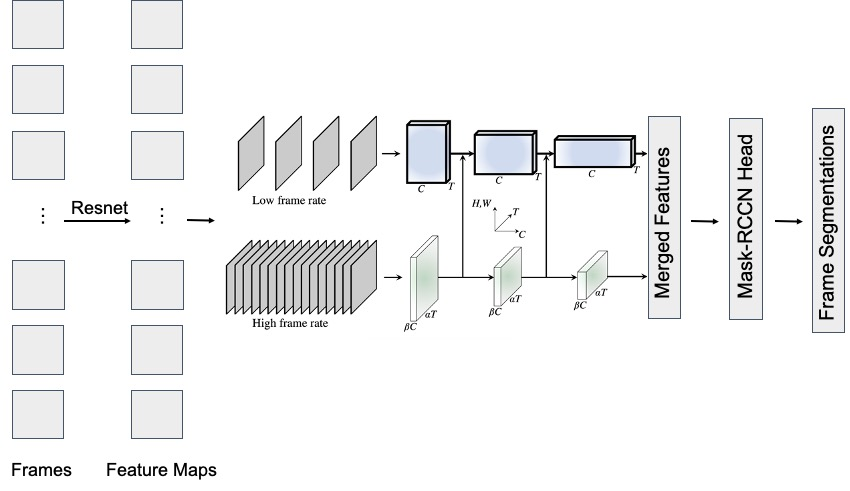
\includegraphics[width=1.8\columnwidth]{OurArchitecture.jpg}
	\caption{SlowFast inspired Video Object Segmentation Architecture for DAVIS dataset.}
	\label{fig:slowfastadapted}
\end{figure*}
\newpage

\bibliographystyle{plain}
\bibliography{literature}


\end{document}
